\section{OpenAPI Specifications and Documentation Drift}

Test validity, discussed above, concerns whether a piece of code's behavior matches what was actually intended. This section addresses a related concern one level removed from the code itself: whether that behavior stays accurately described, in an artifact other people and other systems rely on, once the code has changed.

\textbf{What an OpenAPI specification is.} An OpenAPI specification is a structured, machine-readable document that describes an HTTP API's capabilities --- its endpoints, the inputs each one expects, and the responses it returns --- allowing both humans and computer programs to understand what a service offers without needing to read its source code or inspect its network traffic directly. Because the specification is machine-readable rather than free-form prose, it is not only read by developers as documentation; it is also consumed directly by tooling --- generating client code that calls the API automatically, generating interactive documentation pages, or validating that incoming requests match what the API claims to accept.

\textbf{Why a specification and its implementation can diverge at all.} An OpenAPI specification is, in practice, a separate artifact from the code that implements the API it describes --- typically a separate file, written and updated by hand or by a separate generation step, rather than something the programming language itself enforces consistency with. Nothing structurally prevents the two from disagreeing: a specification file has no built-in awareness that the code it describes has changed, and the code has no built-in awareness that a specification file describing it exists at all, unless something is explicitly built to connect the two.

\textbf{Documentation drift.} This divergence --- between what a specification claims about a system and what the system actually does --- is generally referred to as documentation drift, and its underlying cause is structural rather than accidental: code changes are continuously exercised by compilers, automated tests, and continuous integration pipelines, so problems introduced into the code tend to be caught quickly, while documentation changes are not subject to any of these automatic checks and are instead updated manually, opportunistically, and often incompletely. This is conceptually the same shape of problem as the architectural drift discussed earlier --- a gradual gap opening between an intended, documented state and the actual one --- except here the divergence is not within the code itself, but between the code and a separate document describing it.

\begin{figure}[H]
    \centering
    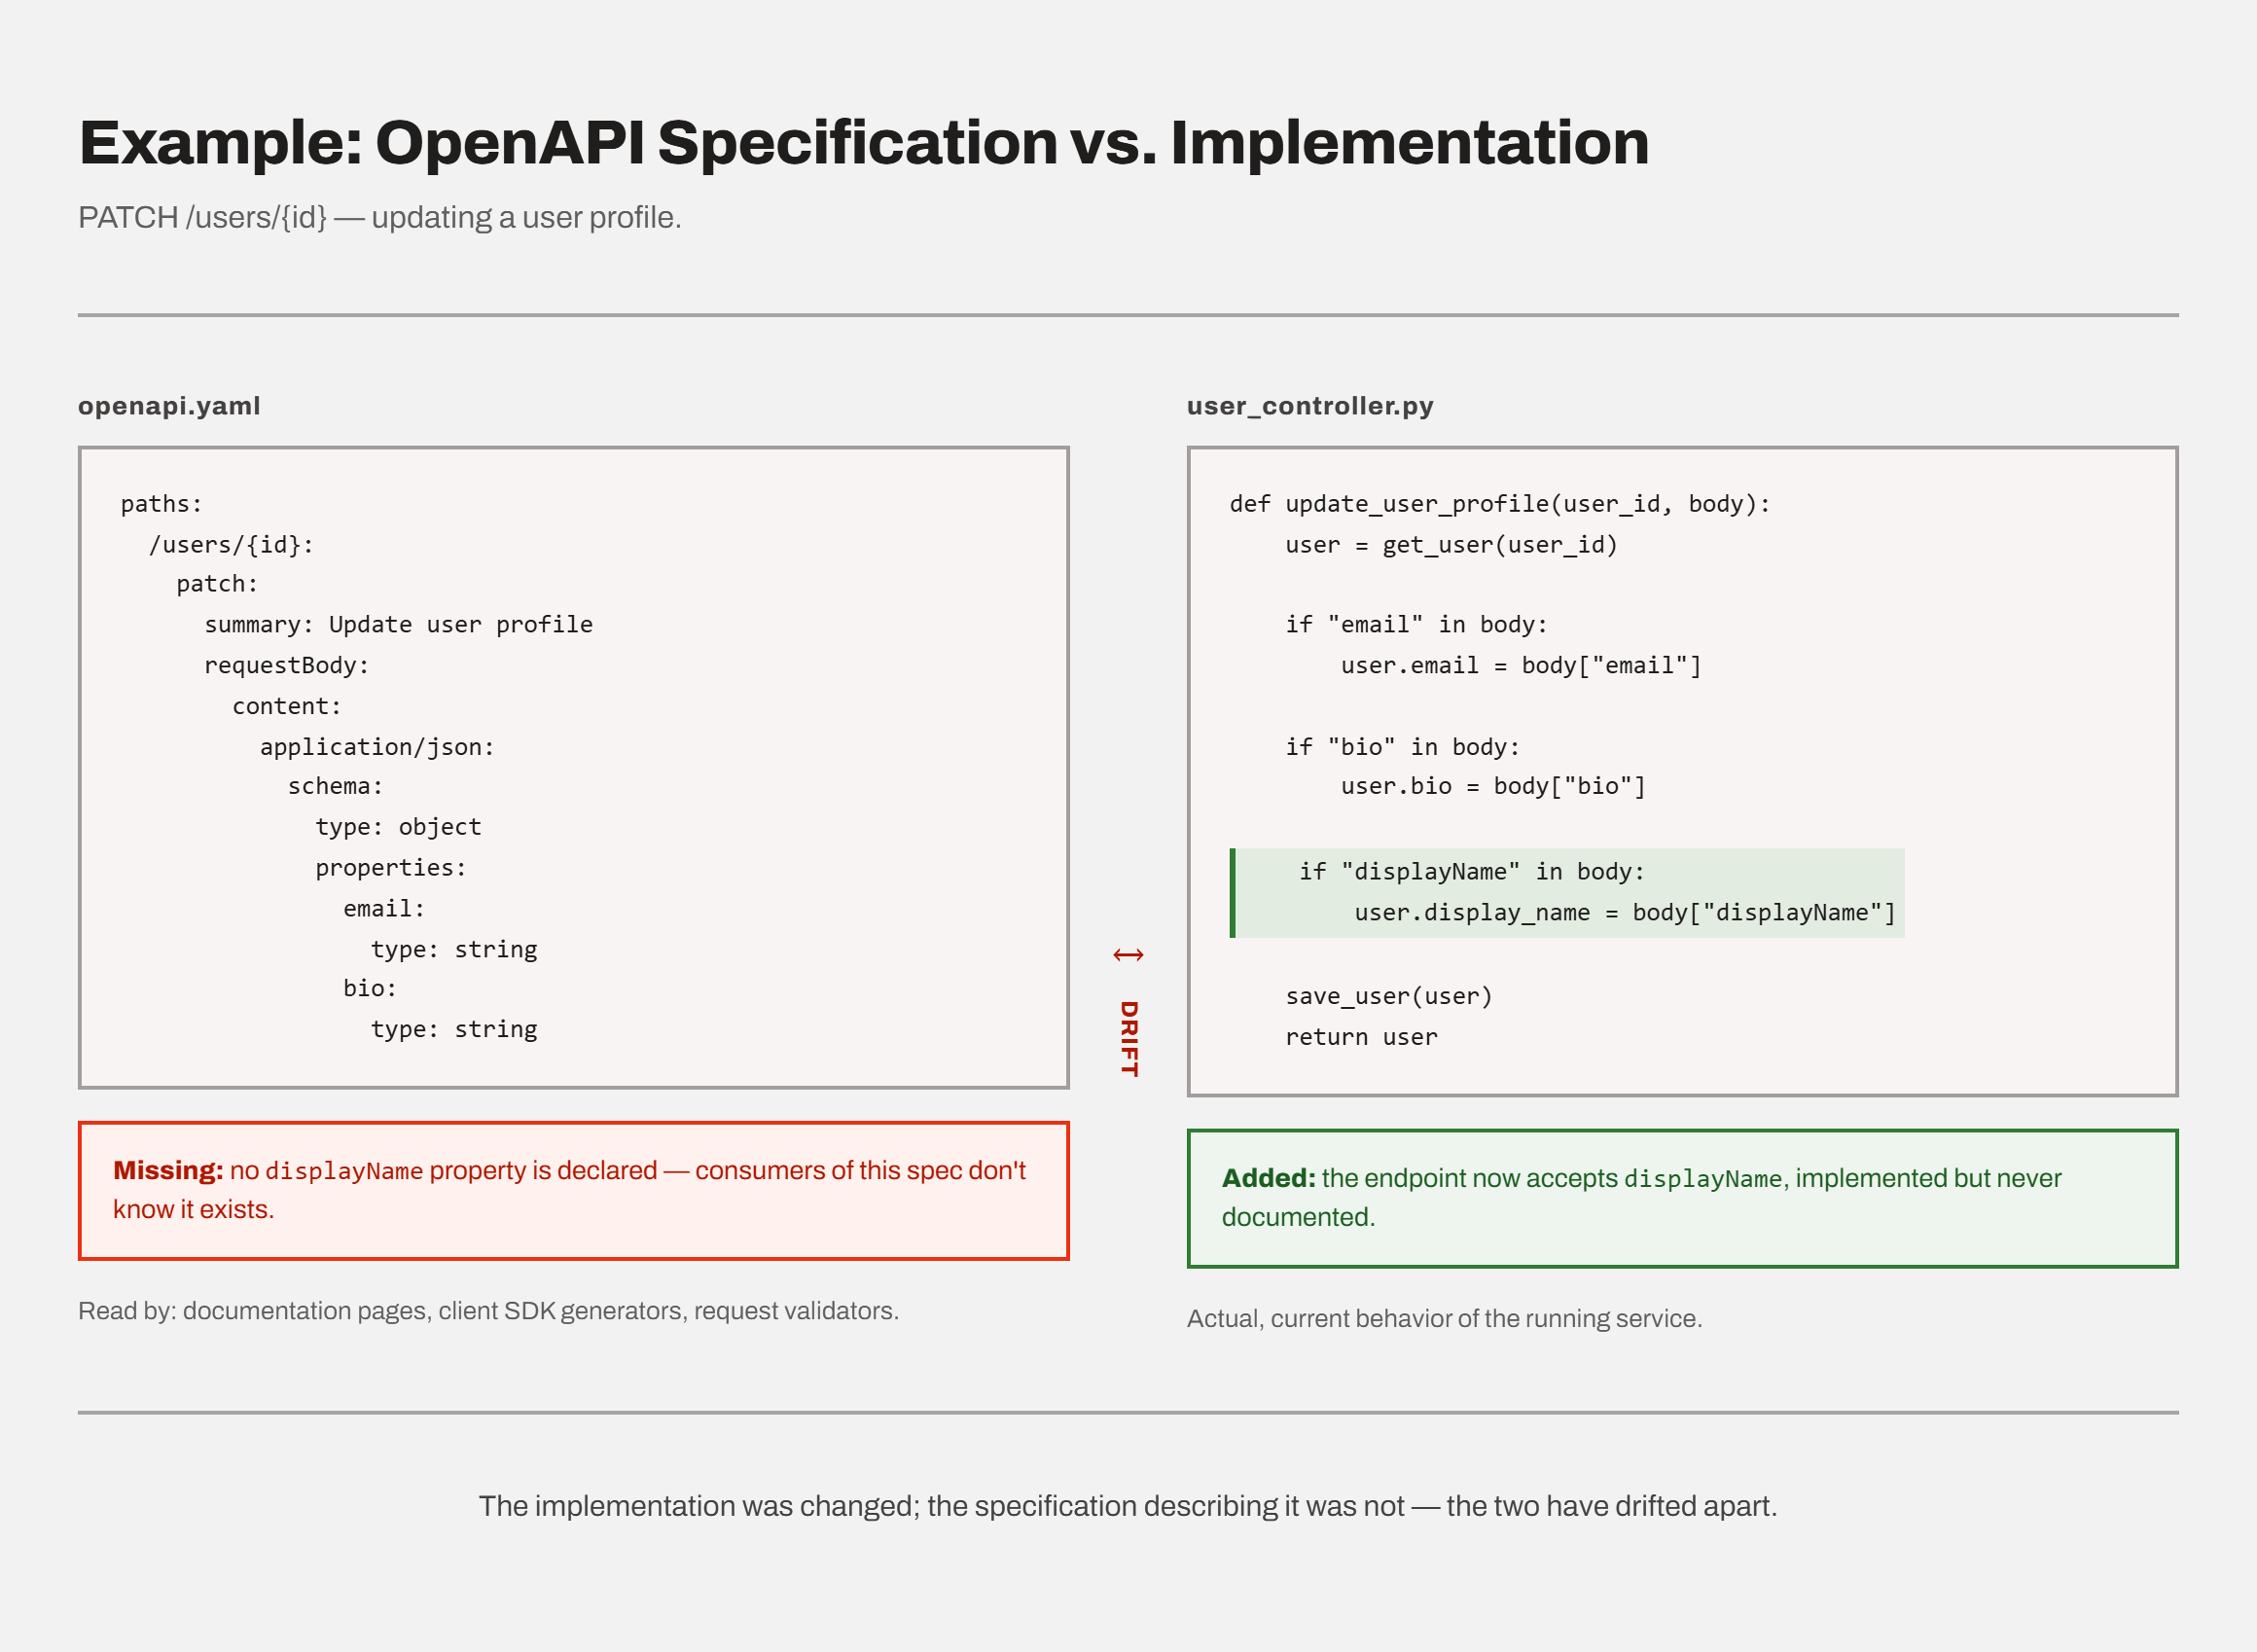
\includegraphics[width=0.82\linewidth]{Bilder/Foundations/documentation-drift.png}
    \caption{An implementation change accepted by the code but never reflected in the OpenAPI specification describing it.}
    \label{fig:documentation-drift}
\end{figure}

\textbf{A concrete illustration.} Suppose an agent is instructed to add a new optional field to an existing endpoint's request body --- for instance, allowing a user profile update to optionally include a display name. Implementing this change means modifying the code that handles the request. Updating the OpenAPI specification to reflect that this new field now exists is a separate, additional step, and nothing about the instruction to "add the field" inherently requires the agent to also touch the specification file, unless it is explicitly told to or has been given a reason to check. If it is not, the implementation now accepts a field the specification does not mention --- a consumer relying on the specification, whether a human developer or an automatically generated client, has no way of knowing the field exists at all, or may be shown an inaccurate picture of what the endpoint actually expects or requires.

\textbf{Why this matters beyond documentation itself.} With OpenAPI specifications specifically, a stale specification is not only a misleading document for a human reader --- because these specifications frequently drive automated tooling directly, a specification that no longer matches the implementation can cause that tooling to actively misbehave: an auto-generated client built from the outdated specification may fail to send the new field at all, or a request-validation step may reject genuinely valid requests because the specification it is checking against has not been updated to allow them.

Like architectural drift, documentation drift is not something a single correctly specified instruction can prevent on its own --- updating an implementation and updating its specification are two separate actions, and nothing automatically ties the two together across the many separate tasks that touch an API over the course of a project, unless something is deliberately built to keep them linked.

